\subsection{RATS}
RIPS was used to scan PHP code, mainly for security-related programming errors.

\subsubsection{Online Banking }
RATS did not show any problems with the PHP code of Online Banking application.

\subsubsection{SecureBank}
RATS reported 5 issues in the PHP code of SecureBank, out of which 1 was of high severity. See \ref{fig:rats_overview_secure_bank}.
The issue was with the usage of the \code{mail} function of PHP. However, upon analyzing the code, it was found that the parameters to the function were not derived from user input. Hence this turned to be a false positive.
The other low severity suspicions were also confirmed to be false positives after manual code inspection.

\begin{figure}[ht]
	\centering
	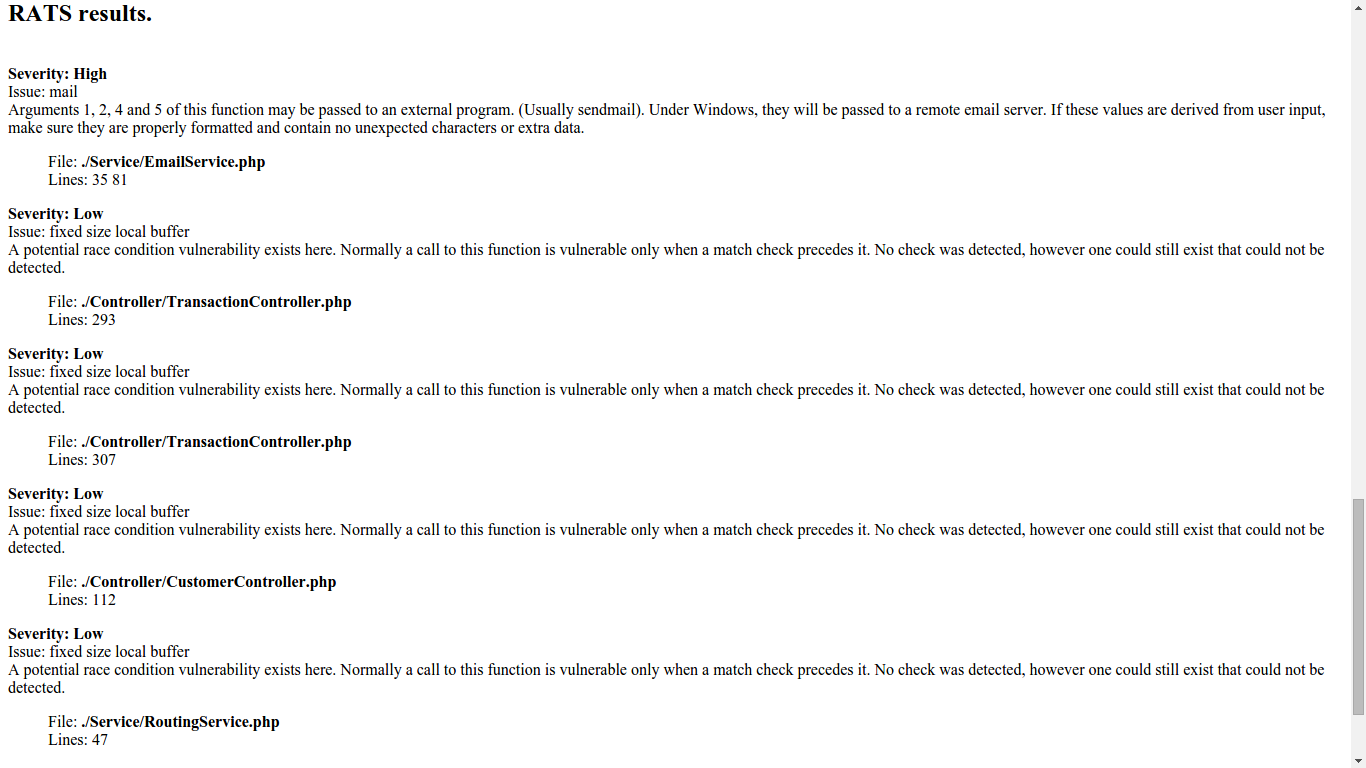
\includegraphics[width=.8\linewidth]{figures/rats_overview_secure_bank.png}
	\caption{Overview of RATS scan for SecureBank}
	\label{fig:rats_overview_secure_bank}
\end{figure}